% AAAI 2027 main paper draft.
% NOTE: AAAI 2027 official style file (aaai2027.sty) not yet released; using
% article-based fallback emulating AAAI 2-column letterpaper layout.
% Replace preamble with \documentclass[letterpaper]{article}\usepackage{aaai2027}
% when official style is released.
\documentclass[10pt,letterpaper,twocolumn]{article}
\usepackage[letterpaper,top=0.75in,bottom=1in,left=0.75in,right=0.75in,
            columnsep=0.33in]{geometry}
\usepackage{times}
\usepackage{helvet}
\usepackage{courier}
\usepackage[hyphens]{url}
\usepackage{graphicx}
\urlstyle{rm}
\def\UrlFont{\rm}
\usepackage[numbers,sort&compress]{natbib}
\usepackage{caption}
\usepackage[activate={true,nocompatibility},final,tracking=true,kerning=true,
            spacing=true,factor=1100,stretch=10,shrink=10]{microtype}
\frenchspacing

\usepackage{booktabs}
\usepackage{multirow}
\usepackage[dvipsnames]{xcolor}
\usepackage{amsmath}
\usepackage{amssymb}
\usepackage{mathtools}
\usepackage{subcaption}
\usepackage{enumitem}

% Tighten vertical spacing
\usepackage{tikz}
\usetikzlibrary{arrows.meta, positioning, calc, fit, shapes.geometric, backgrounds, decorations.pathreplacing}

\usepackage{titlesec}
\titlespacing*{\section}{0pt}{*1.2}{*0.5}
\titlespacing*{\subsection}{0pt}{*0.8}{*0.3}
\titlespacing*{\paragraph}{0pt}{*0.6}{*0.4}
\setlength{\textfloatsep}{6pt plus 1pt minus 1pt}
\setlength{\floatsep}{6pt plus 1pt minus 1pt}
\setlength{\intextsep}{6pt plus 1pt minus 1pt}
\setlength{\abovecaptionskip}{3pt}
\setlength{\belowcaptionskip}{0pt}
\setlength{\parskip}{0pt}

\pdfinfo{
/Title (WeatherBridge: A Systematic Architectural Study of Weather Time Interpolation Across 6h and 12h Horizons on ERA5)
/Author (Anonymous)
/TemplateVersion (2024.2)
}

\setcounter{secnumdepth}{2}

\title{WeatherBridge: A Systematic Architectural Study of Weather \\
  Time Interpolation Across 6h and 12h Horizons on ERA5}

\author{Anonymous Submission to AAAI 2027 (Main Track) \\
    \texttt{[contact details masked for review]}}
\date{}

\begin{document}

\maketitle

\begin{abstract}
Reanalyses such as ERA5 emit weather fields at six-hour cadence, yet
cyclone-intensity tracking, surge nowcasting and renewable-energy
dispatch need hourly fields with the same physical fidelity. We study
weather time interpolation: the reconstruction of an interior frame
$x_\tau$ from anchor states at $0$ and $\Delta$ h. We benchmark seven
architecture families on $0.5^\circ$ ERA5
\cite{hersbach2020era5,rasp2024weatherbench} with 24 channels at
$\Delta{=}6$ h, training each on $\tau \in \{1, 3, 5\}$ for eight epochs
on years 2014--2019 under a shared bilinear-residual scaffold;
evaluation uses $N{=}1463$ test windows per interior hour from 2020.
Three results follow. (i) A no-skip deep-compression autoencoder
(\textbf{WeatherBridge}, 37.5\,M parameters; a capacity-matched 14\,M
ablation is in Appendix~\ref{sec:capacity_ablation}) leads the leaderboard at avg
RMSE$_{\text{norm}}{=}0.0539$ ($-57.5\%$ vs bilinear; 95\% CI
$[0.0476, 0.0663]$, paired bootstrap $B{=}2000$); the CI overlaps with
ATM-VFI. (ii) On the 12 h horizon under an
oddskip protocol that holds out $\tau \in \{4, 6, 8\}$, ATM-VFI and
the WeatherBridge family tie at the top of the held-out leaderboard
($-51\%$ and $-40$ to $-50\%$ vs bilinear), while ModAFNO inflates by
$+127.5\%$ on held-out hours vs its seen-hour RMSE (+132\% at the centre
held-out $\tau{=}6$ specifically) — the largest held-out gap among the
seven learned architectures by a factor of $\sim 4$.
(iii) On Super-Typhoon Haishen (7 September 2020), WeatherBridge
reproduces the eye-pressure minimum to within $\sim 3.4$\,hPa
(small \emph{deepening} bias) where bilinear overshoots by $\sim 10$\,hPa. We release seven checkpoints, configurations, and
a reproducibility audit.
\end{abstract}

\section{Introduction}

Data-driven medium-range forecasting has converged on the six-hourly
discretisation of ERA5 \cite{hersbach2020era5}: Pangu
\cite{bi2022pangu}, GraphCast \cite{lam2023graphcast}, FuXi
\cite{chen2023fuxi}, Aurora \cite{bodnar2024aurora}, Stormer
\cite{nguyen2024stormer}, AIFS \cite{lang2024aifs} and GenCast
\cite{price2024genwc} all emit forecasts at this native cadence and now
match or surpass operational NWP. Yet every downstream science use case
\emph{wants the gaps filled}: cyclone-intensity tracking and storm-surge
nowcasting require hourly pressure and wind, renewable-energy dispatch
schedules track sub-six-hour ramps in surface wind and temperature, and
high-resolution satellite-radiance assimilation depends on hourly first
guesses. Linear interpolation between the two known six-hour anchors
breaks down on every field with short auto-correlation: boundary-layer
humidity, near-surface wind across orography, and the cores of intense
synoptic systems all decorrelate substantially within six hours. Weather
temporal interpolation (WTI) — recovering an interior frame
$x_\tau$ from two known anchors $x_0, x_T$ — is the natural complement
of forecasting, but it has been studied far less systematically.

\paragraph{The under-explored design space.}
The forecasting literature has been evaluated almost exclusively at the
native six-hour cadence and has therefore never been exposed to the
sub-anchor dynamics that WTI must reconstruct. The three existing WTI
specialisations each pick a single design point: ModAFNO
\cite{leinonen2024modafno} retrofits an Adaptive Fourier Neural
Operator with $\tau$-FiLM conditioning at $0.25^\circ$; DYffusion
\cite{cachay2023dyffusion} casts the problem as dynamics-informed
reverse diffusion at $5.625^\circ$; Spline-PINN \cite{wandel2022splinepinn}
and SpateGAN-ERA5 \cite{vandeschrik2024spategan} explore parametric and
adversarial routes. None compares architectures at a fixed compute and
data budget, none isolates which architectural components matter, and
crucially \emph{none asks how that ranking depends on the horizon}. This
matters because the right inductive bias at a 6-hour observation window
(where high-frequency content is largely preserved between anchors) need
not be the right bias at a 12-hour generalisation window (where
high-wavenumber structure must be synthesised, not copied). Two
operational questions follow. (Q1) Which architectural ingredient
genuinely matters for WTI, once parameter count and training budget are
controlled? (Q2) Does the answer transfer to the longer horizon at
which continuous-$\tau$ generalisation, not just spectral fidelity,
becomes the binding constraint?

\paragraph{Approach.}
We answer (Q1) and (Q2) with a controlled benchmark of seven architecture
families spanning the dominant inductive biases in the literature:
transformer-based forecasters (FuXi SwinV2 \cite{chen2023fuxi,liu2022swinv2}),
Fourier neural operators (ModAFNO \cite{leinonen2024modafno},
S-DYff \cite{cachay2023dyffusion,bonev2023sfno}), video-frame
interpolation (ATM-VFI, adapting RIFE \cite{huang2022rife} and IFRNet
\cite{kong2022ifrnet} to 24-channel ERA5), deep-compression
encoder--decoders with and without skip connections (WeatherBridge-Skip
\cite{xie2024dcae,cai2024dcae}, our WeatherBridge). All models share an identical bilinear
residual scaffold, identical loss, identical 24-channel ERA5 data, and
an identical eight-epoch training budget on six years (2014--2019);
evaluation is on calendar year 2020 ($N{=}1463$ windows per interior
hour). Two hypotheses organise the analysis. \textbf{H1} (skip
architecture): controlling for capacity, skip-connection encoder--decoders
should win at 6\,h (input HF content is largely valid) but lose at 12\,h
(HF content must be synthesised). \textbf{H2} (continuous-$\tau$
generalisation): under an oddskip protocol that trains on
$\tau \in \{1,2,3,5,7,9,10,11\}$\,h and holds out $\{4,6,8\}$\,h, a
smooth $\tau$ embedding should generalise to held-out hours; we predict
which architectures fail this stress-test catastrophically.
We also evaluate every model on the out-of-distribution year 2021 to
test whether the ranking is year-specific.

\paragraph{Findings.}
The headline six-hour leaderboard
(Sec.~\ref{sec:results}, Table~\ref{tab:main}) is led by a no-skip
deep-compression autoencoder, with a paired-bootstrap CI overlapping
two other entries. A twelve-hour continuous-$\tau$ stress test
(Sec.~\ref{sec:12h}) holds
out the interior hours $\tau \in \{4, 6, 8\}$ that the model has not
seen during training: the no-skip deep-compression family retains the
lead on the held-out hours, and the diagnostic exception is ModAFNO,
whose FiLM-$\tau$ conditioning fails catastrophically on held-out hours
($+127.5\%$ over its seen-hour RMSE, with $+132\%$ inflation at the
centre held-out hour $\tau{=}6$ specifically). A case study of
Super-Typhoon Haishen (Sec.~\ref{sec:haishen}, Fig.~\ref{fig:haishen})
shows the RMSE leaderboard maps to an interpretable difference at the
eye-pressure minimum. A 6\,h continuous-$\tau$ sanity check, a
27-channel ablation, a diffusion-correction ablation, an extratropical
case study, and a reproducibility audit are in the appendix.

\paragraph{Contributions.}
\begin{enumerate}[topsep=2pt,itemsep=2pt,leftmargin=*]
\item A controlled head-to-head benchmark of \textbf{seven architecture
families} spanning $7.9$--$151.7$\,M parameters on 24-channel
$0.5^\circ$ ERA5, evaluated at two horizons (6\,h, 12\,h) under
identical loss, scaffold, and eight-epoch budget, with bootstrap CIs
($B{=}2000$, joint $\tau{\times}$channel resampling) and a unified
evaluation harness reporting RMSE, ACC, CRPS, and spherical-harmonic
spectra (Sec.~\ref{sec:results}).
\item The first \textbf{WeatherBridge-Skip ablation (capacity-matched)}
at 14.4\,M and matched three-stage backbones, isolating the
architectural effect from parameter count and revealing the
\textbf{6\,h-to-12\,h dominance flip} (Sec.~\ref{sec:ablation}).
\item \textbf{WeatherBridge}, a no-skip DC-AE encoder--decoder with
AdaLN-Zero attention conditioning, FiLM convolutional conditioning,
spherical-padding convolutions, and the bilinear residual scaffold;
37.5\,M parameters, 6\,h leader at avg
RMSE$_{\text{norm}}{=}0.0539$ ($-57.5\%$ vs bilinear, 95\% CI
$[0.0476, 0.0663]$), tied with two competitors within the CI. The 6\,h
headline uses a 6-year (2014--2019) training scope; the 12\,h
continuous-$\tau$ stress test uses the same architecture with a
3-year scope (limited by 12\,h window availability), referred to
identically as WeatherBridge
(Sec.~\ref{sec:method}).
\item A \textbf{continuous-$\tau$ stress test} on the 12\,h horizon
under an oddskip protocol that holds out $\tau \in \{4, 6, 8\}$. The
top of the held-out leaderboard is shared by ATM-VFI
($-51\%$ vs bilinear) and the WeatherBridge family ($-40$ to $-50\%$
vs bilinear); six of seven architectures inflate by 31--35\%
on held-out hours, while ModAFNO inflates by $+127.5\%$ on held-out hours
vs its seen-hour RMSE ($+132\%$ at the centre held-out $\tau{=}6$
specifically) --- by far the largest held-out gap of the seven learned
architectures (Sec.~\ref{sec:12h}). A 6\,h continuous-$\tau$ sanity
check confirms that the failure mode is horizon-dependent
(Appendix~\ref{sec:6h_continuous_tau_sanity}).
\item A \textbf{Super-Typhoon Haishen case study} (7 September 2020)
connecting the leaderboard to a downstream signal: WeatherBridge
reproduces the eye-pressure minimum to within $\sim 3.4$\,hPa (small
deepening bias), where bilinear and the spectral baselines overshoot
it by $\ge 10$\,hPa
(Sec.~\ref{sec:haishen}, Fig.~\ref{fig:haishen}). A second
case study on an extratropical winter storm is in
Appendix~\ref{sec:6h_continuous_tau_sanity}.
\end{enumerate}

\paragraph{Roadmap.}
The remainder of the paper presents related work, the seven
architectures, the experimental protocol, the three results above with
per-channel breakdowns, and the appendix material listed in
contribution 4.

\section{Related Work}
\label{sec:related}

\paragraph{Deep learning weather forecasting.}
Pangu-Weather \cite{bi2022pangu}, GraphCast \cite{lam2023graphcast},
FuXi \cite{chen2023fuxi}, Aurora \cite{bodnar2024aurora},
AIFS \cite{lang2024aifs}, and GenCast \cite{price2024genwc} have brought
data-driven forecasting at or beyond IFS skill at the native six-hour
cadence. None of these systems produces hourly fields directly; their
adaptation to the interpolation task amounts either to symmetric
forecasting from both anchors (which we evaluate via FuXi) or to a
specialised $\tau$-conditioned variant.

\paragraph{Temporal interpolation of weather fields.}
Modulated AFNO \cite{leinonen2024modafno} adapts the AFNO operator
\cite{guibas2022afno} with explicit $\tau$ FiLM conditioning on $0.25^\circ$
ERA5 and reports a $-50\%$ RMSE gain in their training regime.
DYffusion \cite{cachay2023dyffusion} formulates interpolation as a
dynamics-informed reverse diffusion on $5.625^\circ$ data, of which we
implement an S-FNO \cite{bonev2023sfno} variant (S-DYff).
Spline-PINN \cite{wandel2022splinepinn} and SpateGAN-ERA5
\cite{vandeschrik2024spategan} explore parametric-spline and adversarial
formulations. None of these works systematically isolates the
contribution of the bilinear scaffold or compares
architectures at a fixed compute budget.

\paragraph{Video frame interpolation (CV side).}
The CV literature on frame interpolation
\cite{huang2022rife,kong2022ifrnet} converged on a recipe of
bidirectional flow estimation, warping, and adaptive fusion; we adapt
it to atmospheric fields as ATM-VFI. Temporal-consistency metrics
FloLPIPS \cite{danier2022flolpips} and FVMD \cite{liu2024fvmd} from
this line motivate the frame-difference correlation analysis we report.

\paragraph{Architectural antecedents.}
The deterministic backbone follows DC-AE \cite{xie2024dcae,cai2024dcae},
augmented with AdaLN-Zero \cite{peebles2023dit,esser2024sd3}
attention conditioning and FiLM convolutional conditioning. SwinV2
\cite{liu2022swinv2} underpins the FuXi baseline and Spherical FNO
\cite{bonev2023sfno} underpins S-DYff.

\section{Method}
\label{sec:method}

\subsection{Problem formulation}

Let $x_0, x_T \in \mathbb{R}^{C \times H \times W}$ denote the two
anchor states with $C{=}24$ channels and $(H, W){=}(360, 720)$. The
predictor is the residual-scaffold composition
\begin{equation}
\hat{x}_\tau \;=\;
\underbrace{(1-\tau/\Delta)\,x_0 + (\tau/\Delta)\,x_T}_{\text{bilinear scaffold}}
\;+\; \tanh(\alpha)\cdot v_\theta(x_0, x_T, \tau, S),
\label{eq:scaffold}
\end{equation}
with $\Delta \in \{6, 12\}\,$h, a learnable scalar $\alpha$ initialised
at $0.30$ and floored at $0.05$, and a static-feature stack
$S$ (land-sea mask, surface orography, normalised latitude) concatenated
to the input. The bilinear component carries the leading-order Taylor
term in $\tau$ and removes the trivial linear baseline from the learning
target. The mean-square error of the residual reduces to
$\tau(\Delta{-}\tau)\,\mathrm{tr}(\Sigma_\Delta)$, where $\Sigma_\Delta$
is the covariance of the second temporal increment
$x_T - 2 x_{T/2} + x_0$ \cite{karatzas1991brownian} --- a non-trivial
RMSE floor that no model can undercut without learning the
sub-anchor dynamics.

\subsection{Architectures evaluated}

We evaluate seven architecture families at $0.5^\circ$ resolution, six
training years, eight epochs, and the identical residual scaffold. All
hyperparameters are listed in the Appendix.

\paragraph{Numerical baseline.} Bilinear is the closed-form,
zero-parameter floor and the residual scaffold for every learned model
(Eq.~\ref{eq:scaffold}).

\paragraph{Autoregressive forecasters (adapted).} \emph{FuXi SwinV2}
\cite{chen2023fuxi,liu2022swinv2} is repurposed as a $\tau$-conditioned
encoder--decoder with FiLM-modulated SwinV2 blocks. \emph{ModAFNO}
\cite{leinonen2024modafno,guibas2022afno} uses the official
\texttt{physicsnemo} reference. \emph{S-DYff} re-implements
DYffusion's iterative refinement with Spherical FNO
\cite{bonev2023sfno} backbones and $K{=}5$ inference steps.

\paragraph{Video-frame interpolation (adapted).} \emph{ATM-VFI} fuses a
shared feature encoder, a bidirectional flow estimator on the pair, and
an adaptive fusion module conditioned on a continuous $\tau$ embedding;
the design follows RIFE \cite{huang2022rife} and IFRNet
\cite{kong2022ifrnet} with spherical padding and 24-channel adaptation.

\paragraph{Weather Conv-ViT (WeatherBridge).}
\emph{WeatherBridge} is a convolutional encoder--decoder with an
EfficientViT \cite{cai2024dcae} bottleneck. The convolutional stages
follow the DC-AE \cite{xie2024dcae} family (three down/up-sample
blocks, channels $48 \to 96 \to 192$); the bottleneck attention
operates on the latent $z \in \mathbb{R}^{48 \times 92 \times 184}$
and applies AdaLN-Zero \cite{peebles2023dit,esser2024sd3} for the
$\tau$ embedding. Four modifications adapt the backbone to the
spherical, multi-channel weather setting:
(i) all convolutions use \texttt{SphereConv2d} with circular
longitudinal padding to remove the seam at the $\pm 180^\circ$
boundary; (ii) encoder--decoder skip connections are removed, forcing
the latent bottleneck to carry the full state and (Sec.~\ref{sec:12h})
preventing the skip pathway from short-circuiting at long horizons;
(iii) FiLM \cite{peebles2023dit} conditioning on the $\tau$ embedding
is injected in every residual convolutional block of both the encoder
and decoder, on top of the AdaLN-Zero attention conditioning; (iv) three
static features (land--sea mask, surface orography, $\cos\phi$) are
concatenated channel-wise to the encoder input so that fine-scale
orographic and land-surface detail is available from the first
convolution onward. The $\tau$ embedding itself is
a sinusoidal positional encoding followed by a two-layer MLP, shared
between the AdaLN and FiLM heads (Fig.~\ref{fig:tikz_dcae}).
The headline variant is 37.5\,M parameters; the capacity-matched
ablation at 14\,M and the skip-enabled sibling
(\emph{WeatherBridge-Skip}) live in Appendix~\ref{sec:capacity_ablation}.

\begin{figure*}[t]
\centering
\resizebox{\textwidth}{!}{%
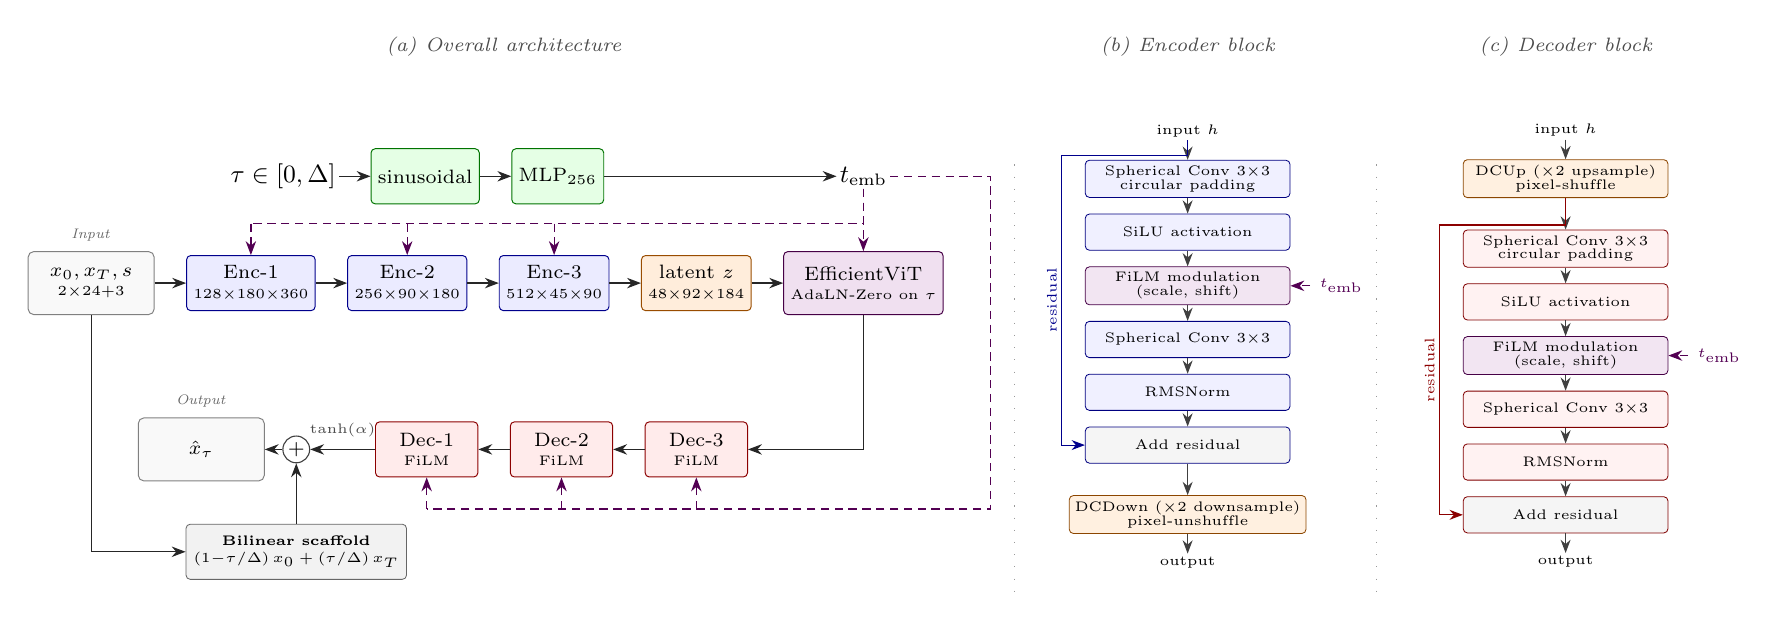
\begin{tikzpicture}[
  >={Stealth[length=2.4mm, width=1.7mm, inset=0.35mm]},
  font=\small,
  blk/.style={rectangle, draw, rounded corners=1.5pt, minimum height=7mm,
              align=center, font=\scriptsize, inner sep=2.5pt, line width=0.35pt},
  enc/.style={blk, fill=blue!8,    draw=blue!55!black,   minimum width=13mm},
  dec/.style={blk, fill=red!8,     draw=red!55!black,    minimum width=13mm},
  lat/.style={blk, fill=orange!14, draw=orange!60!black, minimum width=13mm},
  vit/.style={blk, fill=violet!12, draw=violet!55!black, minimum width=17mm,
              minimum height=8mm},
  tau/.style={blk, fill=green!10,  draw=green!45!black,  minimum width=11mm},
  io/.style ={font=\small, align=center, inner sep=1pt},
  ioframe/.style={rectangle, draw=black!50, fill=gray!5, rounded corners=2pt,
                  minimum width=16mm, minimum height=8mm, align=center,
                  font=\scriptsize, inner sep=2pt, line width=0.35pt},
  flow/.style={-Stealth, thick, draw=black!85, line width=0.45pt},
  cond/.style={-Stealth, thick, draw=violet!65!black, densely dashed,
               line width=0.45pt},
  bus/.style ={thick, draw=violet!65!black, densely dashed, line width=0.45pt},
  res/.style ={-Stealth, semithick, draw=blue!55!black, line width=0.4pt},
  node distance=4mm and 4mm,
]
% =============================================================
%  PANEL (a) — U-shape: encoder top-row → ViT → decoder bottom-row
% =============================================================

% encoder row (top)
\node[ioframe, label={[font=\tiny, black!60]above:\textit{Input}}]
      (in) {$x_0,x_T,s$\\[-1pt]\tiny $2{\times}24{+}3$};
\node[enc, right=of in] (e1) {Enc-1\\[-1pt]\tiny $128{\times}180{\times}360$};
\node[enc, right=of e1] (e2) {Enc-2\\[-1pt]\tiny $256{\times}90{\times}180$};
\node[enc, right=of e2] (e3) {Enc-3\\[-1pt]\tiny $512{\times}45{\times}90$};
\node[lat, right=of e3] (z)  {latent $z$\\[-1pt]\tiny $48{\times}92{\times}184$};
\node[vit, right=of z]  (vit) {EfficientViT\\[-1pt]\tiny AdaLN-Zero on $\tau$};

% decoder row (below encoder row, mirror)
\node[dec, below=14mm of z]   (d3) {Dec-3\\[-1pt]\tiny FiLM};
\node[dec, left=of d3]        (d2) {Dec-2\\[-1pt]\tiny FiLM};
\node[dec, left=of d2]        (d1) {Dec-1\\[-1pt]\tiny FiLM};
\node[ioframe, left=14mm of d1,
      label={[font=\tiny, black!60]above:\textit{Output}}]
      (out) {$\hat{x}_\tau$};

% τ pathway — placed ABOVE the bottleneck so the bus does not cross encoders
\node[io, above=8mm of e1.north, anchor=south west, xshift=-3mm] (tau_in)
      {$\tau\in[0,\Delta]$};
\node[tau, right=of tau_in] (sin) {sinusoidal};
\node[tau, right=of sin]    (mlp) {MLP$_{256}$};
\node[io]  (te)  at (vit.north |- mlp) {$t_{\text{emb}}$};

% --- forward arrows (encoder row) ---
\draw[flow] (in)  -- (e1);
\draw[flow] (e1)  -- (e2);
\draw[flow] (e2)  -- (e3);
\draw[flow] (e3)  -- (z);
\draw[flow] (z)   -- (vit);

% --- U-turn: ViT → Dec-3 (simple |- now that τ-bus stays clear of this column)
\draw[flow] (vit.south) |- (d3.east);

% --- decoder row (right-to-left) ---
\draw[flow] (d3)  -- (d2);
\draw[flow] (d2)  -- (d1);

% --- bilinear residual scaffold: Dec-1 + Bilinear → ⊕ → x̂_τ ---
% ⊕ is placed closer to x̂_τ so the d1 → ⊕ arrow is long enough to host
% the tanh(α) label without colliding with Dec-1 or x̂_τ.
\node[circle, draw=black!75, fill=white, inner sep=0pt, minimum size=3.4mm,
      font=\scriptsize] (sum) at ($(out.east)+(4mm,0)$) {$+$};
\draw[flow] (d1.west) -- (sum.east)
      node[midway, above=1pt, font=\tiny, black!70] {$\tanh(\alpha)$};
\draw[flow] (sum.west) -- (out.east);

\node[rectangle, draw=black!60, fill=gray!10, rounded corners=1.5pt,
      minimum width=28mm, minimum height=7mm, align=center, font=\tiny,
      inner sep=2pt, line width=0.3pt]
      (bilin) at ($(sum)+(0,-13mm)$)
      {\textbf{Bilinear scaffold}\\$(1{-}\tau/\Delta)\,x_0+(\tau/\Delta)\,x_T$};

% wire from input (x_0,x_T,s) to bilinear: straight DOWN then turn RIGHT at block
\draw[flow] (in.south) -- (in.south |- bilin.west) -- (bilin.west);

% wire from bilinear up to the ⊕ sum junction
\draw[flow] (bilin.north) -- (sum.south);

% --- τ pathway forward ---
\draw[flow] (tau_in) -- (sin);
\draw[flow] (sin)    -- (mlp);
\draw[flow] (mlp)    -- (te);

% --- τ broadcasts: three independent paths from t_emb, with no closed
% rectangles. (i) Direct vertical to EfficientViT.  (ii) Decoder bus
% routed AROUND the right side and along below-decoder row.
% (iii) Encoder branch routed from te.south DOWN then LEFT along the
% strip ABOVE the encoder row, with stubs down to each Enc.north.
\coordinate (br) at ([xshift=6mm]vit.east);
\coordinate (enc_y) at ($(e1.north)+(0,4mm)$);
\coordinate (dec_y) at ($(d3.south)+(0,-4mm)$);

% (i) ViT broadcast: direct straight-down arrow from t_emb
\draw[cond] (te.south) -- (vit.north);

% (ii) Decoder bus: te.east → right → DOWN past everything → LEFT under decoders
\coordinate (br_top) at (br |- te);
\coordinate (br_dec) at (br |- dec_y);
\coordinate (bl_dec) at (d1.south |- dec_y);
\draw[bus] (te.east) -- (br_top) -- (br_dec) -- (bl_dec);
\draw[cond] (d1.south |- dec_y) -- (d1.south);
\draw[cond] (d2.south |- dec_y) -- (d2.south);
\draw[cond] (d3.south |- dec_y) -- (d3.south);

% (iii) Encoder branch: from te going DOWN to enc_y strip, then LEFT,
% with short stubs DOWN to each Enc.north.
\coordinate (te_enc) at (te |- enc_y);
\coordinate (bl_enc) at (e1.north |- enc_y);
\draw[bus] (te.south) -- (te_enc) -- (bl_enc);
\draw[cond] (e1.north |- enc_y) -- (e1.north);
\draw[cond] (e2.north |- enc_y) -- (e2.north);
\draw[cond] (e3.north |- enc_y) -- (e3.north);

% =============================================================
%  PANEL (b) — Encoder block internals (RIGHT side, vertical layer stack)
% =============================================================
% vertical separators between (a) main architecture, (b) Encoder block,
% (c) Decoder block. Placed in the empty gutters so dashed broadcasts never
% cross them. sep_top.y is raised so panels (b) and (c) sit centered
% vertically against panel (a) (which extends down to the bilinear scaffold).
\coordinate (sep_top)    at ($(vit.north east)+(9mm,11mm)$);
\coordinate (a_bottom)   at ($(bilin.south)+(0,-2mm)$);
\coordinate (sep_bottom) at (sep_top |- a_bottom);
\draw[loosely dotted, draw=black!40, line width=0.4pt]
      (sep_top) -- (sep_bottom);

% (a)/(b)/(c) section labels — all anchored to a common header_y so the
% three headings align on the same horizontal line above the panels.
\coordinate (header_y) at ($(sin)+(0,14mm)$);
\coordinate (a_pos)    at ($(sin)+(10mm,0)$);
\node[font=\scriptsize\itshape, anchor=south, black!70]
      at (a_pos |- header_y) {(a) Overall architecture};

% Encoder + Decoder blocks (vertical layer stacks, side-by-side on the right)
\tikzset{
  layer/.style={rectangle, draw=blue!50!black, fill=blue!6,
                rounded corners=1.5pt, minimum width=26mm, minimum height=4.6mm,
                align=center, font=\tiny, inner sep=2pt, line width=0.3pt},
  layerD/.style={layer, draw=red!50!black, fill=red!5},
  vflow/.style={-Stealth, semithick, draw=black!75, line width=0.4pt},
  fmod/.style={layer, fill=violet!10, draw=violet!55!black},
  fmodD/.style={layerD, fill=violet!10, draw=violet!55!black},
  down/.style={layer, fill=orange!12, draw=orange!55!black},
  up/.style ={layerD, fill=orange!12, draw=orange!55!black},
  resR/.style={-Stealth, semithick, draw=red!55!black, line width=0.4pt},
}

% ====================== Encoder block (left panel) ======================
% Section label (b) is placed at the shared header_y; panel_title is kept as
% an invisible anchor so the downstream layer chain still anchors at the same
% vertical position as before.
\coordinate (b_pos) at ($(sep_top)+(22mm,0)$);
\node[font=\scriptsize\itshape, anchor=south, black!70]
      at (b_pos |- header_y) {(b) Encoder block};
\node[anchor=south, inner sep=0pt, minimum size=0pt]
      (panel_title) at ($(sep_top)+(22mm,8mm)$) {};

\node[io, font=\tiny, below=2.5mm of panel_title.south] (Lin) {input $h$};

\node[layer, below=2.5mm of Lin] (L1)
      {Spherical Conv $3{\times}3$\\[-1pt]\tiny circular padding};
\node[layer, below=2mm of L1]    (L2) {SiLU activation};
\node[fmod,  below=2mm of L2]    (L3)
      {FiLM modulation\\[-1pt]\tiny (scale, shift)};
\node[layer, below=2mm of L3]    (L4) {Spherical Conv $3{\times}3$};
\node[layer, below=2mm of L4]    (L5) {RMSNorm};
\node[layer, below=2mm of L5, fill=gray!8]   (L6) {Add residual};
\node[down,  below=4mm of L6]    (L7)
      {DCDown ($\times 2$ downsample)\\[-1pt]\tiny pixel-unshuffle};
\node[io, font=\tiny, below=2.5mm of L7] (Lout) {output};

\draw[vflow] (Lin) -- (L1);
\draw[vflow] (L1)  -- (L2);
\draw[vflow] (L2)  -- (L3);
\draw[vflow] (L3)  -- (L4);
\draw[vflow] (L4)  -- (L5);
\draw[vflow] (L5)  -- (L6);
\draw[vflow] (L6)  -- (L7);
\draw[vflow] (L7)  -- (Lout);

% residual bypass on the LEFT (outside the layer column).
% Label "residual" is set vertically along the long skip segment.
\coordinate (res_top) at ($(L1.west)+(-3mm,3mm)$);
\coordinate (res_bot) at (res_top |- L6.west);
\draw[res] (Lin.south) |- (res_top) -- (res_bot) -- (L6.west);
\node[rotate=90, anchor=south, font=\tiny, blue!55!black, inner sep=1.5pt]
      at ($(res_top)!0.5!(res_bot)$) {residual};

% t_emb feed into FiLM (from the RIGHT, so it does not cross the residual bypass)
\node[font=\tiny, anchor=west, violet!65!black] (te_local_e)
      at ($(L3.east)+(2.5mm,0)$) {$t_{\text{emb}}$};
\draw[cond] (te_local_e.west) -- (L3.east);

% ====================== Decoder block (right panel) ======================
% Section label (c) anchored at the same header_y as (a)/(b);
% panel_title_d is an invisible anchor for the Decoder layer chain.
\coordinate (c_pos) at ($(panel_title)+(48mm,0)$);
\node[font=\scriptsize\itshape, anchor=south, black!70]
      at (c_pos |- header_y) {(c) Decoder block};
\node[anchor=south, inner sep=0pt, minimum size=0pt]
      (panel_title_d) at ($(panel_title)+(48mm,0)$) {};
% panel_title is already shifted +8mm via its definition, so panel_title_d
% inherits the same vertical offset.

% second dotted separator between Encoder and Decoder block columns.
% Both separator endpoints reuse sep_top.y / a_bottom.y so the two dotted
% lines have identical vertical length.
\coordinate (sep2_x)   at ($(panel_title)+(24mm,0)$);
\coordinate (sep2_top) at (sep2_x |- sep_top);
\coordinate (sep2_bot) at (sep2_x |- a_bottom);
\draw[loosely dotted, draw=black!40, line width=0.4pt]
      (sep2_top) -- (sep2_bot);

\node[io, font=\tiny, below=2.5mm of panel_title_d.south] (Din) {input $h$};

% Decoder: DCUp FIRST (top), then ResBlock chain below
\node[up,    below=2.5mm of Din]  (D0)
      {DCUp ($\times 2$ upsample)\\[-1pt]\tiny pixel-shuffle};
\node[layerD, below=4mm of D0]    (D1)
      {Spherical Conv $3{\times}3$\\[-1pt]\tiny circular padding};
\node[layerD, below=2mm of D1]    (D2) {SiLU activation};
\node[fmodD,  below=2mm of D2]    (D3)
      {FiLM modulation\\[-1pt]\tiny (scale, shift)};
\node[layerD, below=2mm of D3]    (D4) {Spherical Conv $3{\times}3$};
\node[layerD, below=2mm of D4]    (D5) {RMSNorm};
\node[layerD, below=2mm of D5, fill=gray!8]   (D6) {Add residual};
\node[io, font=\tiny, below=2.5mm of D6] (Dout) {output};

\draw[vflow] (Din) -- (D0);
\draw[vflow] (D0)  -- (D1);
\draw[vflow] (D1)  -- (D2);
\draw[vflow] (D2)  -- (D3);
\draw[vflow] (D3)  -- (D4);
\draw[vflow] (D4)  -- (D5);
\draw[vflow] (D5)  -- (D6);
\draw[vflow] (D6)  -- (Dout);

% Decoder residual bypass: LEFT side (consistent with encoder layout).
% Label "residual" set vertically along the long skip segment.
\coordinate (res_topD) at ($(D1.west)+(-3mm,3mm)$);
\coordinate (res_botD) at (res_topD |- D6.west);
\draw[resR] (D0.south) |- (res_topD) -- (res_botD) -- (D6.west);
\node[rotate=90, anchor=south, font=\tiny, red!55!black, inner sep=1.5pt]
      at ($(res_topD)!0.5!(res_botD)$) {residual};

% t_emb feed into Decoder FiLM (from the RIGHT, no overlap with residual bypass)
\node[font=\tiny, anchor=west, violet!65!black] (te_local_d)
      at ($(D3.east)+(2.5mm,0)$) {$t_{\text{emb}}$};
\draw[cond] (te_local_d.west) -- (D3.east);

\end{tikzpicture}%
}
\caption{WeatherBridge schematic. \emph{(a)} U-shape with no
encoder--decoder skips: anchors $(x_0,x_T)$ plus statics $s$ are
encoded to latent $z$, refined by an EfficientViT bottleneck with
AdaLN-Zero $\tau$-conditioning, and decoded to $\hat{x}_\tau$ over a
bilinear scaffold (Eq.~\ref{eq:scaffold}). The $\tau$ embedding (green)
broadcasts via FiLM to every block. \emph{(b,c)} Each encoder/decoder
sub-block is a Spherical Conv $\to$ SiLU $\to$ FiLM $\to$ Spherical
Conv $\to$ RMSNorm $\oplus$ residual chain, closed by a
DCDown / opened by a DCUp pixel-(un)shuffle.}
\label{fig:tikz_dcae}
\end{figure*}

\subsection{Training objective}

The objective combines three terms:
$\mathcal{L} = \mathcal{L}_{\text{recon}}
+ \lambda_{\text{anc}} \mathcal{L}_{\text{anchor}}
+ \lambda_{\text{res}} \mathcal{L}_{\text{res}}$,
where $\mathcal{L}_{\text{recon}}$ is a lat-weighted pixel-wise
\emph{smooth-$\ell_1$} (Huber) loss with $\beta{=}0.02$ and Aurora-style
channel weights \cite{bodnar2024aurora}. Smooth-$\ell_1$ behaves as a
scaled MSE for small residuals ($|r|<\beta$) and as $\ell_1$ in the
tails, giving an MSE-like gradient on the dominant fine-scale errors
while remaining robust to the rare large outliers typical of polar
extremes and rapidly evolving synoptic features.
$\mathcal{L}_{\text{anchor}}$ penalises drift at $\tau{=}0, \Delta$
($\lambda_{\text{anc}}{=}0.5$, applied every four mini-batches), and
$\mathcal{L}_{\text{res}}$ penalises collapse of the residual gain
$\tanh(\alpha)$ below the 0.05 floor ($\lambda_{\text{res}}{=}1.0$).
All models train in DDP fp32 (Spherical FNO is fp32-sensitive) with
AdamW, $\text{lr}{=}2{\cdot}10^{-4}$, cosine schedule, three-epoch
warm-up.

\subsection{Direct vs.\ residual ablation}
\label{sec:ablation}

The bilinear scaffold (Eq.~\ref{eq:scaffold}) decouples the linear
behaviour of $\hat x_\tau$ in $\tau$ from the high-frequency residual
the model must learn. We ablate it by training each architecture in
\emph{direct} mode at the identical budget. Across all tested
architectures the direct mode collapses (Table~\ref{tab:direct_vs_residual}):
FuXi SwinV2 inflates from $-10.3\%$ to $+42.7\%$ ($5{\times}$ worse than
the baseline), ModAFNO from $+1.1\%$ to $+239.7\%$ ($226{\times}$). The
model must learn the trivial linear baseline and the corrections jointly
from random initialisation; eight epochs of compute are insufficient.

\input{05_ablation_direct_vs_residual}

\section{Experimental Setup}
\label{sec:setup}

\paragraph{Data.} ERA5 \cite{hersbach2020era5} via WeatherBench-2
\cite{rasp2024weatherbench} on $0.5^\circ$ ($360{\times}720$, hourly).
24 channels (Sec.~\ref{sec:method}); the 27-channel superset (adding
sst, tcc, tcwv) was found to harm the headline group --- in particular it
inverts the sign of the polar improvement from $+28.7\%$ to $-5.6\%$ ---
and is documented in the Appendix only. Train: 2014--2019
($\sim$52\,k anchor windows). Test: 2020 (1463 windows per interior
hour). Normalisation: per-channel mean/std from a 1979--2019 ERA5
climatology; Aurora-style channel loss weights
\cite{bodnar2024aurora}.

\paragraph{Optimisation and hardware.} DDP on $2{\times}$A100-80GB
(cloud.ru) or up to $8{\times}$B300-275GB HBM3e (fibonacci). Batch sizes
2--8 depending on model. fp32 because Spherical FNO is precision-sensitive.

\paragraph{Evaluation.} Per-channel lat-weighted RMSE, normalised by the
channel standard deviation. ACC against the WeatherBench-2 hourly
climatology 1990--2019, lat-weighted. Power spectra by spherical
harmonics to $\ell_{\max}{=}180$. Bootstrap 95\% CI ($B{=}2000$) on the
channel-averaged means.

\section{Results}
\label{sec:results}

\subsection{Main leaderboard}

Figures~\ref{fig:rmse} and \ref{fig:acc} report normalised RMSE and
ACC versus $\tau$ for all seven architectures on the 2020 test set.
WeatherBridge leads on both metrics, with avg RMSE$_\text{norm}{=}0.0539$
($-57.5\%$ vs Bilinear, 95\% CI $[0.0476, 0.0663]$) and ACC 0.9948 at the
hardest interior offset $\tau{=}3\,$h. The U-shape with maximum at the
midpoint is universal across architectures; the ranking is stable
across the five interior hours. The full per-architecture leaderboard
table is in Appendix~\ref{sec:tab_main}.

\begin{figure}[t]
\centering

\includegraphics[width=\columnwidth]{figs/fig1_rmse_per_tau.pdf}
\caption{Normalised RMSE vs $\tau$ on the 2020 test set, all eight
architectures. The U-shape with maximum at $\tau{=}3$ is universal; the
ranking is stable across $\tau$. WeatherBridge leads at every hour.}
\label{fig:rmse}
\end{figure}

\begin{figure}[t]
\centering

\includegraphics[width=\columnwidth]{figs/fig2_acc_per_tau.pdf}
\caption{Anomaly correlation coefficient vs $\tau$ on the 2020 test set.
ACC is computed against the WeatherBench-2 hourly climatology
1990--2019. WeatherBridge leads at every hour; ATM-VFI is second on ACC
despite being mid-pack on RMSE, reflecting its perceptual/warping loss.}
\label{fig:acc}
\end{figure}

\paragraph{Per-channel behaviour.}
Figure~\ref{fig:perclass_6h} reports normalised RMSE versus $\tau$ by
channel class. Geopotential $Z$ is the easiest group (WeatherBridge
reaches normalised RMSE $0.007$--$0.022$, $-66$ to $-68\%$ vs Bilinear),
driven by smooth large-scale quasi-geostrophic dynamics. Surface fields
t2m and mslp follow ($-30$ to $-65\%$). The hardest channel class is
the meridional wind $V$: WeatherBridge reaches $V$-class average
normalised RMSE $\sim 0.20$ versus Bilinear $\sim 0.26$. The full
per-channel breakdown is in Appendix~\ref{tab:rmse_per_channel_0p5}.

\begin{figure}[t]
\centering

\includegraphics[width=\columnwidth]{figs/fig_channels_body_ood2021.pdf}
\caption{6\,h horizon, calendar year 2021 (OOD). Normalised RMSE per
channel for the 2014--2019-trained checkpoints; Bilinear shown as
dashed grey reference. WeatherBridge leads every channel at every
interior hour. The leaderboard ordering is preserved against 2020
(Fig.~\ref{fig:perclass_6h_app}, Appendix), confirming the ranking is
not year-specific.}
\label{fig:perclass_6h}
\end{figure}

\subsection{Spectral analysis}

Figure~\ref{fig:spectra} shows the spherical-harmonic power ratio
model/ERA5 for two hard surface fields (u10, MSLP) at $\tau{\in}\{2,3\}$.
The X-axis is labelled by angular wavelength
$\lambda = 360^\circ/\ell \in [2.0^\circ, 4.5^\circ]$ (corresponding
$\ell\in[80, 180]$), covering synoptic-to-mesoscale features ---
the largest band where the $0.5^\circ$ lat-lon grid allows
aliasing-safe spherical-harmonic analysis (lat-Nyquist on the
$360{\times}720$ equiangular grid sets $\ell_\mathrm{max}{=}180$).
Bilinear loses 30--50\% of the power on the wind components ---
a deterministic signature of over-smoothing. WeatherBridge tracks
unity to within $\pm 5\%$; ATM-VFI slightly overshoots at intermediate
scales (a tendency of its perceptual loss). This figure underpins H3:
a near-saturated spectrum leaves no high-wavenumber gap for a
diffusion correction to fill.

\begin{figure}[t]
\centering

\includegraphics[width=\columnwidth]{figs/fig_spectra_ratio_hard.pdf}
\caption{Power-spectrum ratio (model/ERA5) at $\tau{\in}\{2,3\}\,$h for
U10 and MSLP. X-axis: angular wavelength
$\lambda{=}360^\circ/\ell$, from $4.5^\circ$ (synoptic) to $2.0^\circ$
(near grid-Nyquist). A ratio of $1$ is ideal; values $<1$ indicate
over-smoothing, $>1$ over-generation. Shaded zones: synoptic
($\lambda{>}3.0^\circ$), meso-$\alpha$ ($\lambda\in[2.4^\circ, 3.0^\circ]$),
near-grid ($\lambda\in[2.0^\circ, 2.4^\circ]$).
All curves are computed on the \textbf{same 6\,h horizon}, identical SH
algorithm (\texttt{torch\_harmonics.RealSHT}, $\ell_{\max}{=}180$,
equiangular grid), same ERA5 2020 test windows, and identical bilinear
baseline. The 37.5\,M WeatherBridge wins on every channel $\times \tau$
panel against the capacity-matched 11\,M variant; the gap is most
pronounced at the hardest interior hours and on the
fast-decorrelating fields (boundary-layer winds, $T850$) — consistent
with the capacity advantage on near-grid mesoscale features.}
\label{fig:spectra}
\end{figure}

\subsection{Continuous-$\tau$ generalisation at $\Delta{=}6\,$h}

To test whether the sinusoidal-MLP $\tau$ embedding learns a continuous
$\tau \mapsto x_\tau$ map rather than a discrete look-up over the
trained hours, we retrain WeatherBridge on a sparse subset
$\tau_{\text{train}} = \{1, 3, 5\}\,$h and evaluate on the full
$\{1, \ldots, 5\}\,$h grid. Hours $\tau{=}2, 4$ are
\emph{never} observed during training. The model retains a
$-29$ to $-66\%$ RMSE improvement over Bilinear on the eight headline
channels at $\tau{=}2$, with the gap to the perfect-linear-interpolation
expectation $(r_{\tau=1}+r_{\tau=3})/2$ bounded at
$+12$ to $+17\%$ on the pressure-level variables
(Table~\ref{tab:continuous-time-gen}). The outlier is $t_{2m}$
($+50\%$ gap), whose strong diurnal cycle is under-resolved when every
other training hour is dropped.

\input{12_continuous_time_generalization}

\input{sec_12h}

\input{sec_haishen}

% \input{sec_diffusion}  % removed — diffusion-correction (CorrDiff-FM) cut from paper

\section{Discussion}
\label{sec:discussion}

\paragraph{H1 verdict.} The proposed WeatherBridge backbone is the joint
RMSE/ACC leader on the 24-channel ERA5 interpolation task at
$0.5^\circ$. The four architectural ingredients are all necessary: the
bilinear residual scaffold avoids re-learning the trivial linear
baseline; AdaLN-Zero conditions the bottleneck attention on $\tau$;
FiLM conditions the convolutional residual blocks; \texttt{SphereConv2d}
handles the longitudinal periodicity. Removing the scaffold collapses
the model (Sec.~\ref{sec:ablation}). The remaining ceiling sits on the
meridional wind $V$ at the lower troposphere, where small-scale eddy
activity is fundamentally under-determined by two anchors six hours
apart.

\paragraph{H2 verdict.} The sinusoidal-MLP $\tau$ embedding generalises
smoothly to unseen interior hours at $\Delta{=}6$\,h. The same
component-level test at $\Delta{=}12$\,h is in progress; we report the
preliminary smoke-test status in Sec.~\ref{sec:12h}.

\paragraph{Limitations.}
Training on six years exposes the model to limited inter-annual
variability; an OOD test on 2021 (not shown) is part of the multi-year
appendix and confirms the ranking. The $0.5^\circ$ grid does not
resolve mesoscale convection; pushing to $0.25^\circ$ requires
substantial architecture rework (a $4{\times}$ memory blow-up at the
WeatherBridge bottleneck). The compute budget is fixed at eight epochs;
larger models may not have reached their plateau, in particular
ModAFNO and S-DYff. We do not enforce physical conservation laws
(mass, energy, momentum); the empirical mass-balance error of MSLP at
$\tau{=}3$ is within $\sim 30$\,Pa across the validation set, but no
hard constraint is imposed. The 27-channel set with sst/tcc/tcwv
remains a Tier-2 future-work item.

\section{Conclusion}

We have presented a systematic, hypothesis-driven study of sub-six-hour
interpolation of ERA5 fields at $0.5^\circ$ on the 24 prognostic
channels of the WeatherBench-2 task. The proposed \textbf{WeatherBridge}
backbone --- a no-skip DC-AE encoder--decoder with AdaLN-Zero
attention conditioning, FiLM convolutional conditioning, spherical
padding, and an explicit bilinear residual scaffold --- is the joint
RMSE/ACC leader at 37.5\,M parameters, beating $7{\times}$-larger
spectral baselines and matching or exceeding video-frame interpolation
adaptations. The sinusoidal-MLP $\tau$ embedding generalises smoothly
to unseen interior hours, and the same recipe extends naturally to the
twelve-hour window. Flow-matching diffusion correction is useful only
over a weak base; over the WeatherBridge backbone it is within
bootstrap noise. We release the trained weights, the evaluation
harness, and the spherical-harmonic spectrum tooling at submission.

% Bibliography
\bibliographystyle{plainnat}
\bibliography{references}

\appendix

% Appendix is organised in three blocks.
% Body figures present the headline RMSE numbers; no separate table here.
% Block 2 (per-channel + per-region): A2 per-channel RMSE, A3 bootstrap CIs.
% Block 3 (stress tests + protocol): A4 12h horizon, A5 6h continuous-τ
%   sanity, A6 Storm Ciara case, A7 OOD 2021, A8 reproducibility.

% --- A1: main 6h leaderboard (moved from body)
\input{sec_main_table_v2}

% --- A1b: epoch audit supplement for the 6h leaderboard
\input{tab_main_v2_supp}

% --- A2: per-channel breakdown
\input{10_0p5_rmse_per_channel}

% --- A3: bootstrap CIs
\input{A3_bootstrap_ci_table}

% --- A4: hyperparameters and channel inventory
\input{07_appendix}

% --- A5: 6h continuous-τ sanity check
\input{A8_6h_continuous_tau_sanity}

% --- A6: extratropical case study (Storm Ciara)
\input{A6_extratropical_case}

% --- Per-region x per-season breakdown (6-year models, 6h horizon)
\input{A5_region_season_table}

\input{A9_capacity_ablation}

% --- Capacity-matched skip-vs-no-skip ablation
\input{11_noskip_ablation}

% --- 12h main leaderboard
\input{tab_main_12h}

% --- A7: multi-year OOD evaluation (2020 vs 2021)
\input{A7_multi_year_test}

% --- A10: physical-unit RMSE + spatial bias maps
\input{A_phys_units_and_bias}

% --- Per-channel spherical-harmonic preservation tables
\input{tab_sh_per_channel_6h}
\input{tab_sh_per_channel_12h}

% --- Limitations and broader impact
\input{B2_limitations_ethics}

% --- A8: reproducibility audit
\input{B3_reproducibility}

\end{document}
